\section*{KnowledgeGraph}

\begin{frame}
\centerline{\textbf{\Large{KnowledgeGraph}}} 
~\\
\centerline{\large{张永辉}}
\end{frame}

\subsection*{什么是知识图谱}
\begin{frame}
	\begin{itemize}
		\item 知识图谱是表示为图的知识 
			\begin{itemize} 
				\item 每个点表示一个实体(Entity)
				\item 每条边表示一个关系(Relation)
			\end{itemize}
		
		\item 知识图谱中存储的事实是三元组(Head,Relation,Tail)
			\begin{itemize} 
				\item Head:subject entity
				\item Relation:关系类型
				\item Tail: objecti entity
				\item 可以理解为:主、谓、宾
			\end{itemize}
	\end{itemize}
\end{frame}

\subsection*{举个例子}
\begin{frame}
	\begin{itemize}

		\item Donald Trump is a Politician of USA
			\begin{itemize} 
				\item Head: Donald Trump
				\item Relation: isPoliticianOf
				\item Tail: USA
			\end{itemize}
		\item (梁启超,isFatherOf,梁思成)
		\item (梁思成,isSonOf, 梁启超)
		\item (梁思成,isFatherOf,梁再冰)
		\item (林徽因,isMotherOf,梁再冰)
	\end{itemize}
\end{frame}

\begin{frame}
	\begin{figure}[htbp]
		\centering
		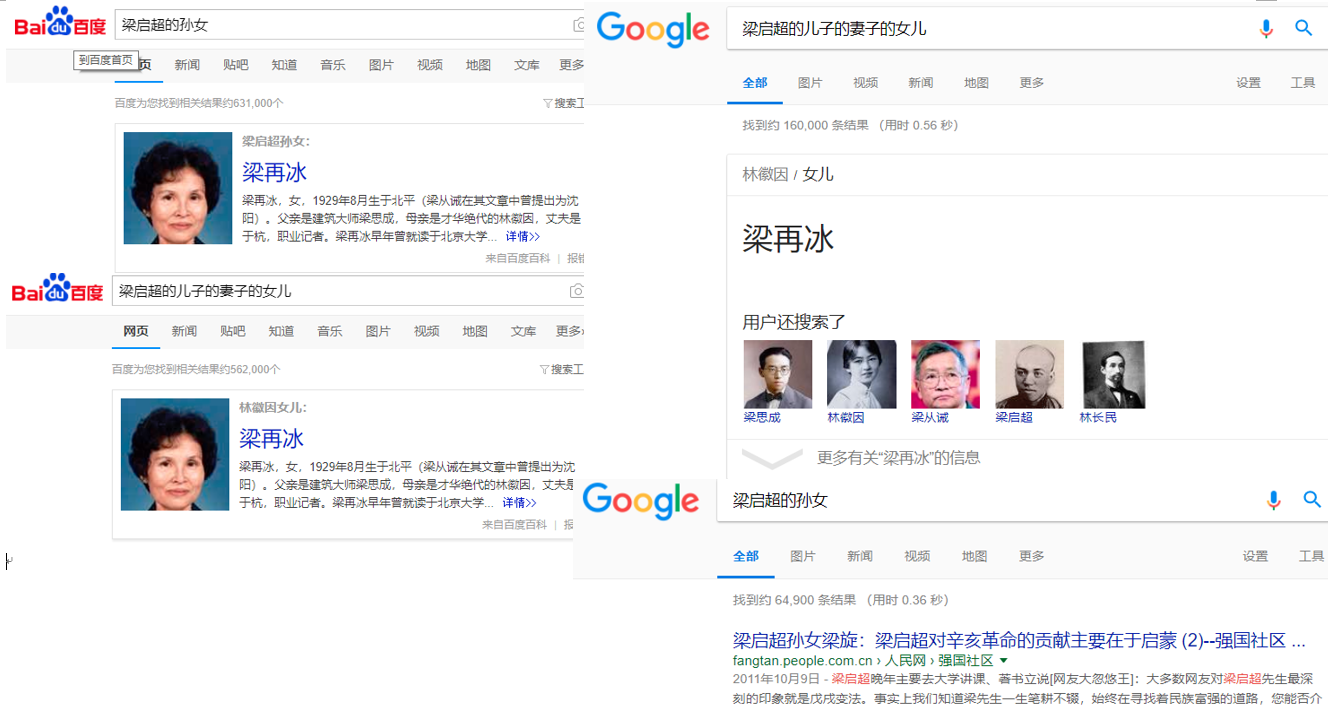
\includegraphics[width=\textwidth, bb= 0 0 1000 400]{pic/kg/kg_example1.png}
%		\caption{放置图片}
%		\label{0-001}
	\end{figure}
\end{frame}

\subsection*{如何生成知识图谱}
\begin{frame}
	\title {如何构建知识图谱}
	\begin{itemize}
		\item 手工构建
		\item 自动构建
		\begin{itemize} 
			\item 知识抽取:抽取实体和实体之间的关系
			\begin{itemize} 
				\item 实体抽取
				\item 关系抽取
				\item 属性抽取(珠穆朗玛峰)
			\end{itemize}
			\item 知识融合:整合相同义项,消歧义
			\item 知识加工:进行质量评估(可能有人工参与)将知识加入到知识库中
		\end{itemize}
	\end{itemize}

\end{frame}

\begin{frame}
	\begin{figure}[htbp]
		\centering
		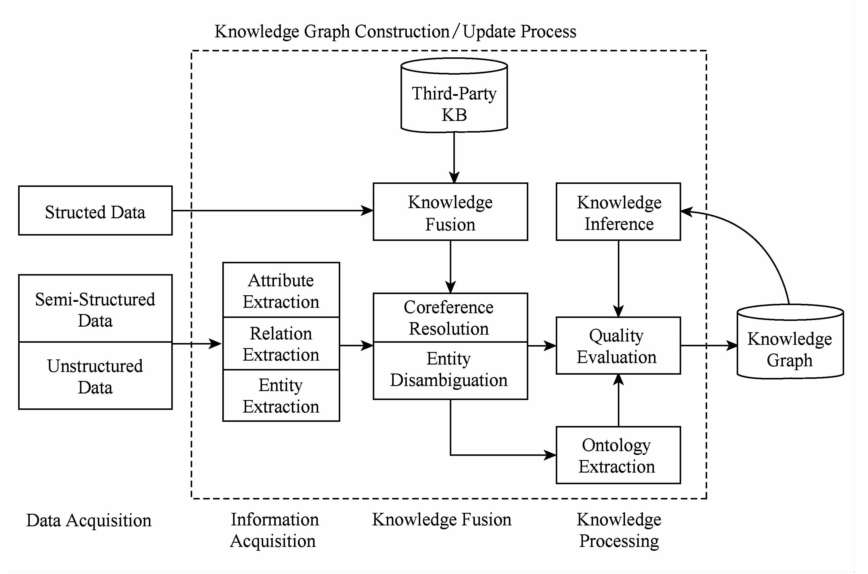
\includegraphics[width=\textwidth, bb= 0 0 600 400]{pic/kg/build_kg.png}
%		\caption{放置图片}
%		\label{0-001}
	\end{figure}
\end{frame}

\subsection*{自动生成错误的例子}
\begin{frame}
	\begin{figure}[htbp]
		\centering
		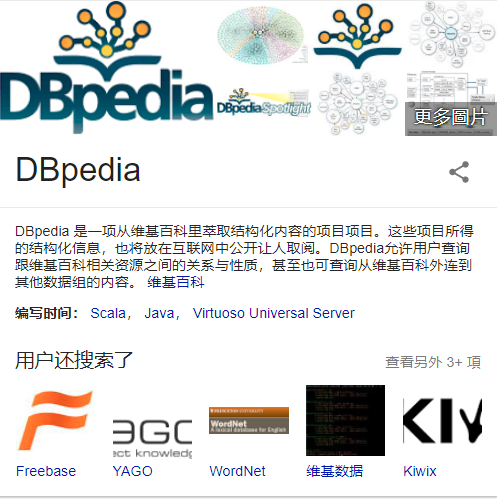
\includegraphics[width=0.5\textwidth, bb=0 0 400 400]{pic/kg/DBpedia_1.png}
		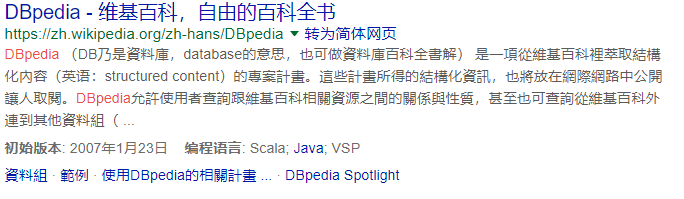
\includegraphics[width=0.5\textwidth, bb=0 0 400 400]{pic/kg/DBpedia_2.png}
	\end{figure}
	\begin{figure}[htbp]
		\centering
		
	\end{figure}
\end{frame}

\subsection*{Representation Learning}

\begin{frame}

	\begin{columns}
		\column{.5\textwidth}
			\begin{itemize}
				\item 之前所讲的是将Knowledge表示为图,但我们还可以表示为向量
				\item 实体是一个高维向量,关系也是一个高维向量			
			\end{itemize}
		\column{.5\textwidth}
			\begin{figure}[htbp]
				\centering
				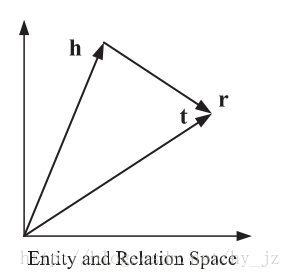
\includegraphics[width=1\textwidth, bb= 0 0 400 400]{pic/kg/transE.png}
			\end{figure}
	\end{columns}
	 
\end{frame}

\begin{frame}
	\title {TransE}
	\begin{itemize}
		\item  给定一个fact(h,r,t),TrasE模型将关系表示为translation 向量 r⃗ ,这样就能以较低的错误把实体的向量$\vec{h}$, $\vec{t}$连接起来,即:$\vec{h} + \vec{r} \approx \vec{t}$。 打分函数定义为:$\vec{h} + \vec{r}与\vec{t}$之间的距离:
		\item 
		\begin{equation}
			f_r(h,t) = -||\vec{h} + \vec{r} - \vec{t}||_{1/2}
		\end{equation}
		\item 其中,$[x]_+$表示$max\{0,x\}$,$\gamma$是margin超参数。根据max-margin的思想,$\mathcal{L}$表示的是负样本的分数最多比正样本高$\gamma$,再大就没有奖励了。也就是说正样本$\vec{h}+\vec{r}$与$\vec{t}$的距离小,负样本的距离大。E是实体的集合,S表示正样本的集合 ,$S^{'}_{(h,r,t)}$是负样本: 	
		\item
			\begin{equation}
			S^{'}_{(h,r,t)}=\{(h^{'},r,t)| h^{'} \in E\} \cup \{ (h,r,t^{'})| t^{'} \in E\}
			\end{equation}
		
	\end{itemize}

\end{frame}

\begin{frame}
	\begin{itemize}
		\item https://blog.csdn.net/hy\_jz/article/details/78944717
		\item 虽然TransE模型简单有效,但是它并不能处理1-N,N-1, N-N的问题。比如,一个导演指导了多部电影,根据头节点h(导演),关系r(指导),尾节点t(电影)进行模型训练,那么这些电影向量的距离是很近的,而事实上他们是完全不同的实体。 
	\end{itemize}
\end{frame}

\begin{frame}
	\begin{itemize}
		\item TransH —— TransE的问题所在是,在任何relation下实体的向量表示都是相同的,这就造成了以下两点: 1. 如果 $(h,r,t) \in fact$并且$(t,r,h) \in fact$,也就是说r是一个自反的映射,那么$\vec{r} = \vec{0} $并且 $\vec{h} = \vec{t}$; 2. 如果r是一个N-1的映射,$\forall i \in {0, \cdots , m} (h_i , r,t)$,那么$\vec{h}_0= \cdots = \vec{h}_m$;同样的,如果r是一个1-N的映射,$\forall i \in {0, \cdots , m} (h , r,t_i)$,那么$\vec{t}_0= \cdots = \vec{t}_m TransH$ 依然把实体 h,t 表示为向量,但是把关系r表示成两个向量:超平面的法向量 $\vec{W}_r$和关系r在超平面内的向量表示 $\vec{d}_r$。如下图所示:	
	\end{itemize}
\end{frame}
\begin{frame}
\begin{figure}[htbp]
	\centering
	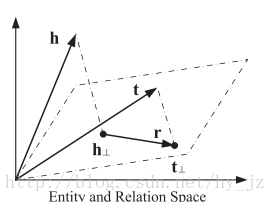
\includegraphics[width=0.6\textwidth, bb= 0 0 277 202]{pic/kg/transH.png}
\end{figure}
头结点h和尾节点t映射到超平面的表示为: 
\begin{equation}
\vec{h}_{\perp} = \vec{h} - \vec{W}_r^T \vec{h} \vec{W}_r \quad  \vec{t}_{\perp} = \vec{t} - \vec{W}_r^T \vec{t} \vec{W}_r 
\end{equation}
\end{frame}

\subsection*{如何推理}

\begin{frame}
	\begin{itemize}
		\item 传统推理
			\begin{itemize}
				\item 机器证明
			\end{itemize}
		\item 基于知识图谱(图)的推理
		\item 基于分布式表示(向量)的推理
		\item 基于神经网络的推理
	\end{itemize}
\end{frame}

\subsection*{问题}
\begin{frame}
\begin{itemize}
	\item 如何在小样本中学习知识图谱
	\item 如何建立对时间敏感的知识图谱
		\begin{itemize}
			\item \(Who,isPresidentOf,USA\)
			\item Obama
			\item D.T. Trump
		\end{itemize}
\end{itemize}
\end{frame}